\section{Integration Experiments}
\label{text:experiments/integration}
In the following, the performance of the overall approach is evaluated. For comparison, several baselines have been re-implemented, that are frequently used in the field of crowd navigation: \ac{ORCA} \cite{vandenBerg2011}, \ac{RRT}$\star$ \cite{Karaman2011} and \ac{MCTS}. These baselines have been chosen, as they cover a broad field of existing trajectory planning methodologies, such as sampling-based, optimization-based or tree-search-based methods.\footnote{Section \ref{text:related/crowd_navigation} introduced the use of deep learning-based approaches in the field of crowd-navigation. Therefore, a state-of-the-art approach for socially-aware navigation using deep reinforcement learning, by Chen et alt. \cite{Chen2017}, should have been used as well. Unfortunately, it is neither open-source nor did the author reply to several of my requests.} The experiments have been conducted as described in Section \ref{text:experiments/setup}, using \ac{SGAN} \cite{Gupta2018} as independent simulation environment and averaged of several runs in an Monte-Carlo manner.

\subsection{Effect of Interactive Objective}
Figure \ref{img:show_case} illustrates the qualitative difference between the proposed approach and other planning approaches. Note that meanwhile both algorithms can maintain some safety distance to the pedestrian. However, integrating the pedestrian prediction in the core of the optimization allows the solver to anticipate future actions of each pedestrian. While the path optimized by \ac{RRT}$\star$ (comp. Figure \ref{img:show_case}, right) cuts into the path of the green-colored pedestrian, the interactive-aware optimization chooses to stay behind the pedestrian, which is reasonable travel-time efficient but introduces a lot less disturbances on the surrounding pedestrians. 

\begin{figure}[!ht]
\begin{center}
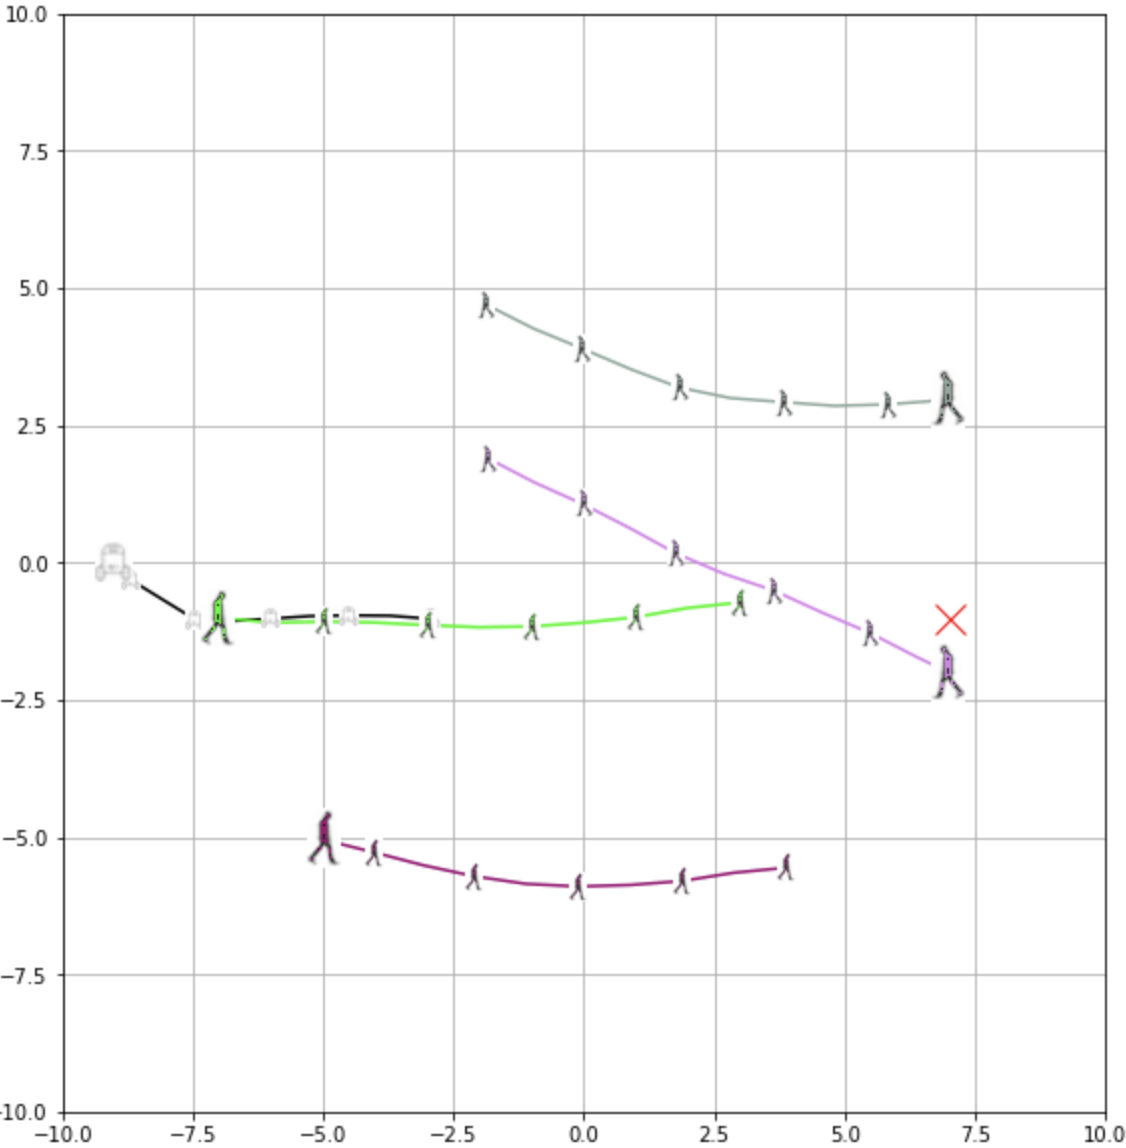
\includegraphics[width=0.45\textwidth]{images/show_case_ipopt.png}
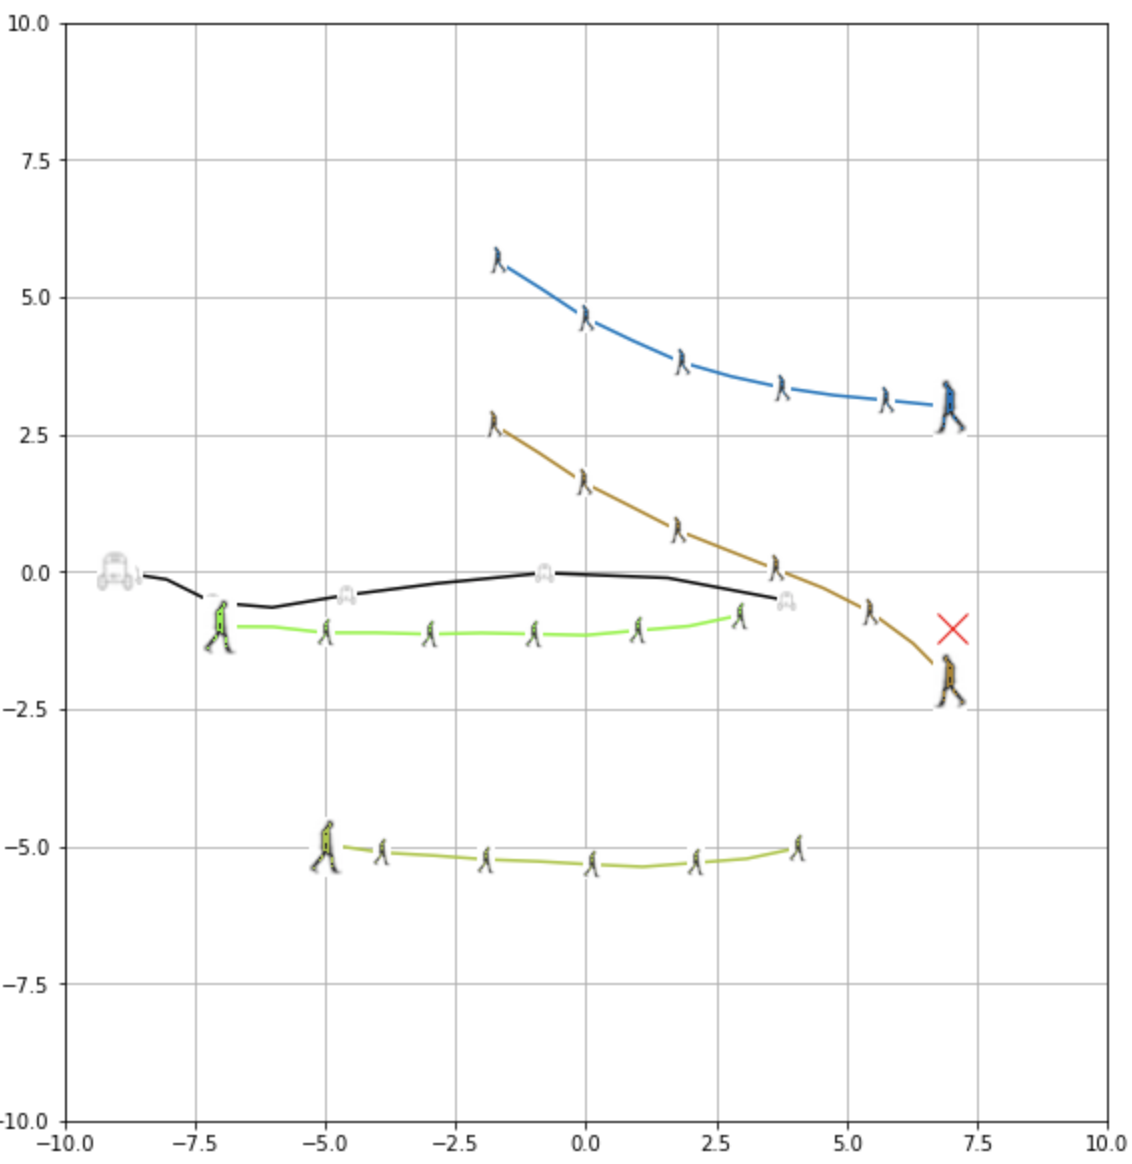
\includegraphics[width=0.45\textwidth]{images/show_case_rrt.png}
\end{center}
\caption{Direct comparison of generated trajectories by our approach (left) and \ac{RRT}$\star$ \cite{Karaman2011} (right)}
\label{img:show_case}
\end{figure}

\subsection{Baseline Performance}
The previously described qualitative benefits of the proposed approach can be underlined by quantitative results. The following experiments compare the quantitative results of the several planning algorithms, in the presence of 2 to 5 pedestrians in the scene and each one randomly created. 

\subsection{Effect of number of Pedestrians}
Figure \ref{img:runtime_num_pedestrian} illustrates the average algorithm's runtime for one trajectory optimization, in dependence of the number of pedestrian. While the proposed approach ("ipopt") runs with about 2 Hz, the runtime is notably depends only marginally on the number of pedestrians in the scene. This can be explained by the comprehensive usage of batching within the algorithm, including the prediction model, and the use of attention filters, which keep the number of considered pedestrians during optimization approximately constant.

\begin{figure}[!ht]
\begin{center}
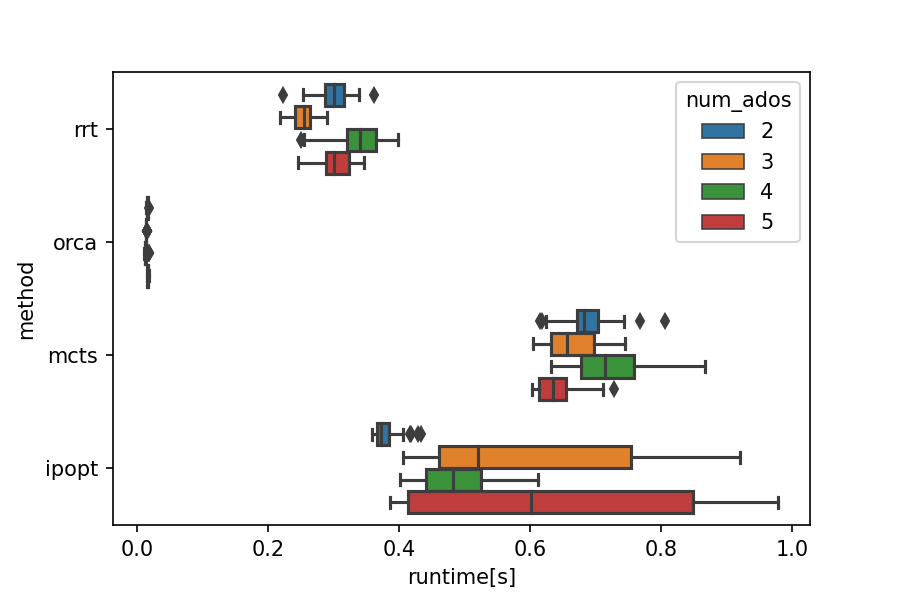
\includegraphics[width=\imgwidth]{images/runtime_peds.png}
\end{center}
\caption{Impact of number of pedestrians (ados) on algorithm runtime [s].}
\label{img:runtime_num_pedestrian}
\end{figure}

\subsection{Effect of Prediction Model}

